% ATTENTION 
% ce modèle a été compilé avec la ligne de commande et le script «bashcommandeCompilation.sh» inclus dans le dossier These. 
% Ceci a grandement facilité la compilation des différents chapitres et leurs bibliographiesrespectives. 
% Sinon il faut s'assurer de compiler manuellement chacun des chapitres et de rouler bibtex pour chacun d'eux, ceci dans le même ordre que spécifié dans le script bash. 
% Ce modèle répond aux exigences du Département de Biologie en date de Février 2021. 
% Ce code produit TheseRef.pdf qui inclut chaque bibliographie par chapitre et la bibliographie générale. 

\documentclass[12pt,oneside,x11names,svgnames,table]{book}
\usepackage[a-1b]{pdfx}
\usepackage[T1]{fontenc}
\usepackage[utf8]{inputenc}
\usepackage{lipsum}

%\includeonly{chapitre1}  	%pour inclure seulement quelques chapitres dans la compilation (et faire des tests)


%-------------------LANGUE ET BIBTEX----------------------------
\usepackage[a4paper]{geometry}
\usepackage{mathpazo} 			% utilise Palatino pour les mathématiques (mettre en premier)
\usepackage{newtxtext, newtxmath} 	% utilise la police Times Roman
\usepackage[sectionbib]{natbib}	% avant BABEL
\usepackage{chapterbib}			% avoir plusieurs bibliographies dans le même document avec la commande \include 
\usepackage[french]{babel}  		% comment this line if the thesis is in English
\usepackage{hyperref}
\setlength{\bibhang}{0pt}			% aucune indentation dans les bibliographies  
\setlength{\bibsep}{10pt}			% 1 interligne et demi entre les entrées de la bibliographie
%%% Uncomment if you want to include the bibliographies at the end of each chapter in the table of contents.  
%\usepackage[nottoc]{tocbibind}


%-------------------FORMAT----------------------------
\usepackage{lineno}			% ajoute des numero de ligne (pour PREMIER DÉPÔT SEULEMENT - COMMENTER POUR DÉPÔT FINAL)
\usepackage{pdflscape}		% permet d'avoir des page horizontale (utile pour grande table large)
\usepackage[section]{placeins}	% ajoute la commande \FloatBarrier qui empêche les figure de trop bouger	
\usepackage{graphicx}		% gère l'insertion des figures
\usepackage{setspace} 		% gère l'interligne
\usepackage{amsfonts}		% ajoute des polices mathématiqueS
\usepackage{amsmath}             % ajoute des environnements mathématiques
\usepackage{mathrsfs}		% ajoute une meilleure police calligraphique pour certains symboles
\usepackage{gensymb}		 % gère les symboles
\usepackage{xcolor}


%% page en format paysage avec numéro de page en bas, centré 
\usepackage{everypage}
\newlength{\hfoot}
\newlength{\vfoot}
\AddEverypageHook{\ifdim\textwidth=\linewidth\relax
\else\setlength{\hfoot}{-\topmargin}%
\addtolength{\hfoot}{-\headheight}%
\addtolength{\hfoot}{-\headsep}%
\addtolength{\hfoot}{-.5\linewidth}%
\ifodd\value{page}\setlength{\vfoot}{\oddsidemargin}%
\else\setlength{\vfoot}{\evensidemargin}\fi%
\addtolength{\vfoot}{\textheight}%
\addtolength{\vfoot}{\footskip}%
\raisebox{\hfoot}[0pt][0pt]{\rlap{\hspace{\vfoot}\rotatebox[origin=cB]{90}{\thepage}}}\fi}

%-------------------FIGURES ET TABLEAUX ----------------------------
\usepackage{subcaption}		 % pour mettre des figures côte à côte 
\usepackage[format=hang,justification=raggedright,labelfont=bf, singlelinecheck = false, font=bf, labelsep=quad]{caption}	% modifie la manière dont les descriptions de tableaux et figures sont disposées
\usepackage{epsfig} 			% ajouter et convertir figures .eps. Ne pas mettre l'extension dans le document 
\usepackage[most]{tcolorbox}
\usepackage[flushleft]{threeparttable} % notes de bas de tableau 
\usepackage{adjustbox}			 % gère les gros tableaux 
\usepackage{tabularx, multirow,booktabs}


%------------------COMPILATION PDFLATEX----------------------------
\newif\ifhyper\hypertrue  	% options PDF. Requiert de compiler avec pdflatex
%\hyperfalse 			% décommenter pour supprimer les hyperliens (version imprimée)
\ifhyper\usepackage[pdfa]{hyperref} 
\urlstyle{same}
\hypersetup{ 
     backref=true, pagebackref=true,   % ajoute les liens dans la bibliographie
     hyperindex=true, 		% ajoute des liens dans les index. 
     colorlinks=true, 		% colore les liens 
     breaklinks=true,		% permet le retour la ligne dans les liens trop longs 
     urlcolor= black,  		% couleur des hyperliens (doit inclure x11names dans xcolor ci-dessus)
     linkcolor= black, 		% couleur des liens internes 
     citecolor=black,		% couleur des liens de citation
     bookmarks=true,		% créationŽŽ des signets PDF 
     bookmarksopen=true,	% ouvre les signets PDF au départ 
}\else\relax\fi

%-------------------PAGINATION ----------------------------

\makeatletter			% ENLÈVE LA PAGINATION DES PREMIÈRES PAGES DE SECTIONS
\renewcommand\chapter{\if@openright\cleardoublepage\else\clearpage\fi
                    \thispagestyle{empty}%
                    \global\@topnum\z@
                    \@afterindentfalse
                    \secdef\@chapter\@schapter}
\makeatother


%------------------FORMAT DES CHAPITRES----------------------------
\pagestyle{plain} 		% Entêtes et pieds % pas d'entête, no de page en bas
\usepackage{titlesec}	% Format de titres de chapitres, sections et sous-sections
\newcommand\chapterstring{CHAPITRE}

%\titleformat{command to change}[shape of the title]{format of the title}{label of the title}{space between label and title}{code preceding the title body}[code following the title body]
%\titlespacing*{command to change}{left space}{space with paragraph before the title}{space with paragraph after the title}[right space]


% Règle 2.4.5 
% Entre la numérotation du chapitre et le titre du chapitre, introduire un changement de ligne (1 ½ interligne).
\titleformat{\chapter}[display]{\vspace{-6em}\bfseries\center}{\chapterstring~\thechapter}{0pt}{}
\titleformat{\section}{\normalfont\bfseries}{\thesection}{10pt}{}
\titleformat{\subsection}{\normalfont\bfseries}{\thesubsection}{10pt}{}
\titleformat{\subsubsection}{\normalfont\normalsize\bfseries}{\thesubsubsection}{10pt}{}
\titleformat{\paragraph}[runin]{\normalfont\normalsize\bfseries}{\theparagraph}{10pt}{}
\titleformat{\subparagraph}[runin]{\normalfont\normalsize\bfseries}{\thesubparagraph}{10pt}{}


% Après le titre d'un chapitre, le premier titre ou paragraphe du dit chapitre se trouvera à quatre interlignes et demi du titre (36 pts).
\titlespacing*{\chapter}{0pt}{36pt}{36pt} 

% Trois interlignes (ou 24 pts) séparent les titres des sous-titres ou des paragraphes, les sous-titres des paragraphes, les paragraphes des sous-titres et les paragraphes entre eux.
\titlespacing*{\section}{0pt}{24pt}{24pt}
\titlespacing*{\subsection}{0pt}{24pt}{24pt}
\titlespacing*{\subsubsection}{0pt}{24pt}{24pt}
\titlespacing*{\paragraph}{0pt}{24pt}{24pt}
\titlespacing*{\subparagraph}{0pt}{24pt}{24pt}


%------------------MARGE DU DOCUMENT ---------------------------

\geometry{letterpaper,lmargin=1.0in,rmargin=1in,tmargin=1.5in,bmargin=1.0in}
\setlength{\parindent}{0ex} 	% indentation au début de chaque paragraphe
%\setlength{\parskip}{3ex plus 0.3ex minus 0.1ex} % espace vertical entre paragraphes
%\setlength{\parskip}{12pt}
\usepackage{nowidow}


%-------------------SAUTS DE PAGE, FORMAT TABLE DES MATIÈRES ET LISTES ----------------------------
\newcommand{\blankpage}{	% page blanche au tout début du document 
\newpage
\thispagestyle{empty}
\mbox{}
\newpage
}
% table des matières
\usepackage[titles]{tocloft} 	 
\usepackage{calc} 
\renewcommand{\cftchapleader}{\cftdotfill{\cftdotsep}} % Ligne pointillée entre titre de chapitre et # de page


% ceci personnalise la table des matières avec les noms de chapitre, leur numéro ainsi que leur titre, incluant un "-" 
% une macro fait la même chose aux appendixes 
\renewcommand{\cftchappresnum}{CHAPITRE\space}
\setlength{\cftchapnumwidth}{\widthof{\textbf{Appendix~999~}}}
\renewcommand{\cftchapaftersnum}{  -- }
\makeatletter
\g@addto@macro\appendix{%
  \addtocontents{toc}{%
    \protect\renewcommand{\protect\cftchappresnum}{ANNEXE\space}%
        \protect\renewcommand{\protect\cftchapaftersnum}{}%

  }%
}

% pour les annexes : ne pas inclure les numéros de sections dans la TOC mais garder la numérotation pour les figures 
\appto\appendix{\addtocontents{toc}{\protect\setcounter{tocdepth}{0}}}

% reinstate the correct level for list of tables and figures
\appto\listoffigures{\addtocontents{lof}{\protect\setcounter{tocdepth}{1}}}
\appto\listoftables{\addtocontents{lot}{\protect\setcounter{tocdepth}{1}}}


% format liste de figures
\newlength{\mylen}
\renewcommand{\cftfigpresnum}{Figure\enspace}
\renewcommand{\cftfigaftersnum}{\hspace{1mm}}
\settowidth{\mylen}{\cftfigpresnum\cftfigaftersnum}
\addtolength{\cftfignumwidth}{\mylen}

%format liste de tableaux
\newlength{\mylent}
\renewcommand{\cfttabpresnum}{Table\enspace}
\renewcommand{\cfttabaftersnum}{\hspace{1mm}}
\settowidth{\mylent}{\cfttabpresnum\cfttabaftersnum}
\addtolength{\cfttabnumwidth}{\mylent}


\newcommand*{\noaddvspace}{\renewcommand*{\addvspace}[1]{}}
\addtocontents{lof}{\protect\noaddvspace}	% diminue l'espace entre les items de la liste 
\addtocontents{lot}{\protect\noaddvspace}


%------------------CORPS DU DOCUMENT----------------------------

\begin{document}
%\raggedbottom 	% éviter un étirement bizarre
\blankpage
\blankpage


%-------------------------------------------------------------------------------
%  FRANCISER LES TERMES DE LA PRESENTATION
%-------------------------------------------------------------------------------
\renewcommand{\figurename}{Figure}
\renewcommand{\tablename}{Table} 		% TABLEAU EN FRANÇAIS 
\renewcommand{\chaptername}{CHAPITRE} 
\renewcommand{\contentsname}{TABLE DES MATIÈRES}
\renewcommand{\listtablename}{LISTE DES TABLEAUX}
\renewcommand{\listfigurename}{LISTE DES FIGURES}


%------------------PAGE TITRE----------------------------

\thispagestyle{empty}
\singlespacing
\begin{center}
{
%\sffamily 	% commenter cette ligne pour un lettrage en roman, avec sérif
{\textbf{Mécanismes de flux d'énergie en interactions trophiques}} % titre
\\  \vspace{2.5cm}
par
\\   \vspace{2.5cm}
{\textbf{Benjamin Mercier}} % inscrire votre nom
\\   \vspace{2.5cm}
Mémoire présenté au Département de biologie en vue\\
de l'obtention du grade de maître ès sciences (M.Sc.)\\
\vfill
FACULTÉ DES SCIENCES\\
UNIVERSITÉ DE SHERBROOKE\\  \vspace{1.5cm}
\vfill
Sherbrooke, Québec, [mois et année du dépôt final]
}

\end{center}


%------------------PAGE DE COMPOSITION DU JURY ----------------------------

\blankpage
\thispagestyle{empty}
\singlespacing
\begin{center}
%\vglue 1cm
Le [date du dépôt final]\\   \vspace{1cm} % à changer
\textit{Le jury a accepté le mémoire de [Madame ou Monsieur (optionnel)] Benjamin Mercier dans sa version finale.}\\  \vspace{1cm}
Membres du jury\\  \vspace{1cm}

Professeur Dominique Gravel\\
Directeur de recherche\\
Département de Biologie\\
Université de Sherbrooke\\ \vspace{13mm}

Professeur[e] [Prénom et nom]\\
Codirectrice ou Codirecteur de recherche\\
Département [nom]\\
Nom de l'institution\\ \vspace{13mm}

[Pour le doctorat seulement]\\
Professeur[e] [Prénom et nom]\\
Évaluatrice ou Évaluateur externe\\
Département [nom]\\
Nom de l'institution\\ \vspace{13mm}

Professeur[e] [Prénom et nom]\\
Évaluatrice ou Évaluateur interne\\
Département [nom]\\
Nom de l'institution\\ \vspace{13mm}

Professeur[e] [Prénom et nom]\\
Président-rapporteur\\
Département de biologie\\
Université de Sherbrooke\\ \vspace{13mm}
\end{center}



%------------------PREMIER DÉPÔT ----------------------------
\linenumbers 	% ajoute des numero de ligne (pour PREMIER DÉPÔT SEULEMENT - COMMENTER POUR DÉPÔT FINAL)


%------------------REMERCIEMENTS ----------------------------
\blankpage
%\onehalfspacing
\setstretch{1.3} 		% un peu plus que 1.5 pour que ça concorde avec Word
\chapter*{REMERCIEMENTS} 
Je tiens d’abord à remercier mon directeur Dominique Gravel. Mon comité. Andrew et Willian. Le laboratoire d'écologie intégrative. Finalement, ma famille sans qui cette grande avanture n'aurait jamais été possible. Merci pour tout.


%------------------SOMMAIRE ----------------------------
%\parskip 1.2in % added by me
\blankpage	% commenter si vous ne souhaitez pas une page impaire ici

\pagenumbering{roman}	% en chiffre romain
\chapter*{SOMMAIRE}
\setcounter{page}{9} 		% ATTN spécifier manuellement où commence la numérotation des pages APRÈS LES REMERCIEMENTS et SELON LES PAGES BLANCHES
Inclure ici un résumé global de la maîtrise.
\vfill{}
\textbf{Mots clés :} réseaux trophiques, interactions, flux d'énergie


%\blankpage			% decommenter si table des matières est sur page impaire


%------------------INCLURE TABLE DES MATIÈRES ET FIGURES ----------------------------
{
\setlength{\parskip}{0ex}
\cleardoublepage
\phantomsection 	% INCLUT TABLE DES MATIÈRES, SANS "TABLE DES MATIÈRES" DEDANS
\tableofcontents
}
\cleardoublepage
\listoftables

\cleardoublepage
\listoffigures


%------------------SIGLES ET ABRÉVIATIONS ----------------------------
\cleardoublepage
\chapter*{LISTE DES ABRÉVIATIONS ET DES SIGLES}

\begin{tabular}{ ll } 
 MGE & Modèle Général d'Écosystème \\
 \end{tabular}

 

%------------------CITATIONS----------------------------

\renewenvironment{quote}
  {\singlespacing\small\list{}{\rightmargin=2.5cm \leftmargin=2.5cm}%
   \item\relax}
  {\endlist}
  
  
%------------------CORPS DU DOCUMENT ----------------------------

\mainmatter
%\onehalfspacing
\setstretch{1.3} 
\chapter{\textbf{INTRODUCTION}}
Insérer ici un paragraphe intéressant global et accrocheur.

\begin{quote}
« All models are wrong, but some are useful.»\\
-- George Box
\end{quote}

\section{Mise en contexte}
Parler des modèles globaux d'écosystème (MGE).

\section{Le jeu de données}
\subsection{Nature des données}
Les données proviennent de l'étude de Jacquet.
\subsection{Distribution globale}
Voici la distribution globale des réseaux utilisés. 


\FloatBarrier
\begin{figure}[!htb]
\centering
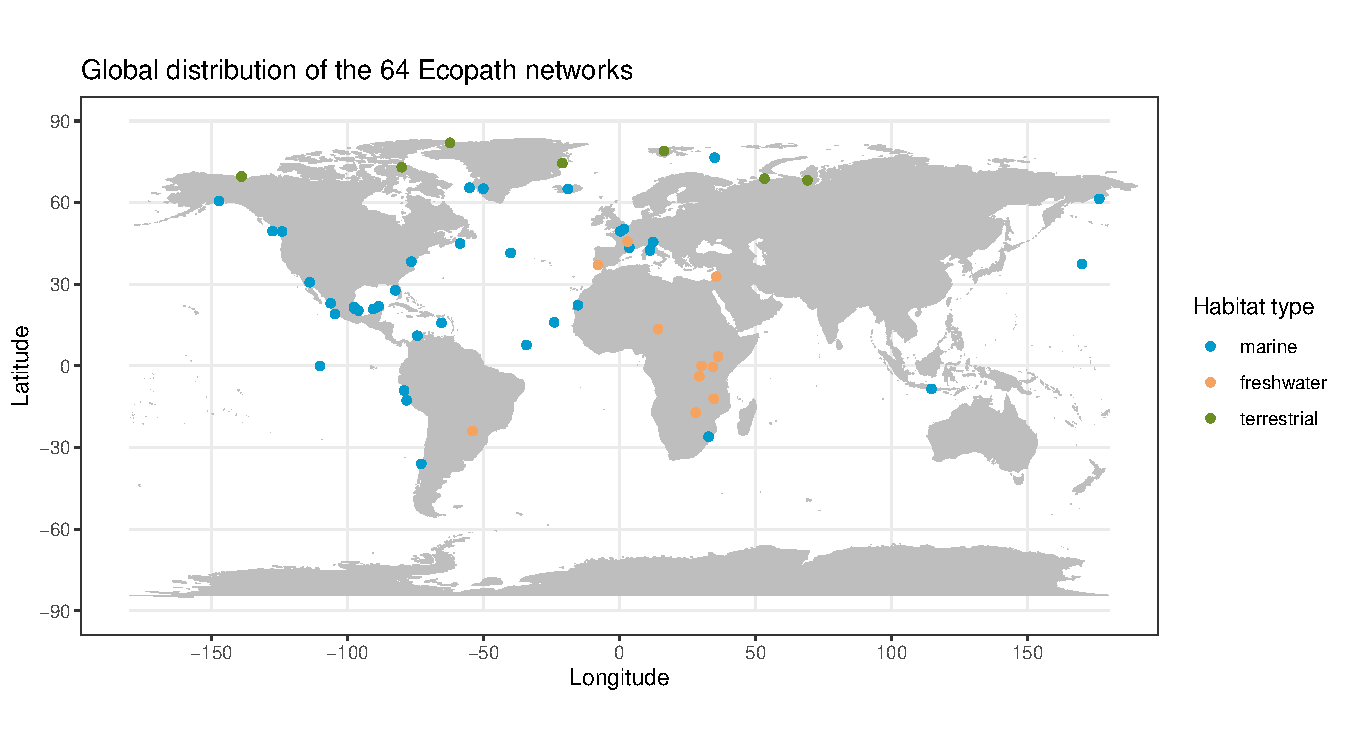
\includegraphics[width=\textwidth]{figs/chapitre1/network_map.pdf} % ici mettre le répertoire exact de la figure - Dossier Thèse, sous-dossier figs - chapitre 1
\caption[Titre de figure]{
Distribution des réseaux Ecopath \par{}
\smallskip		% saut de ligne entre titre et légende de figure
\normalfont{Légende de figure} 
}
\label{reaction_norms}
\end{figure}




% ajouté ceci pour faire un test 
% cite correctement dans le texte mais plus à la fin générale du document
%\singlespacing 
%{\renewcommand{\bibname}{References}
%\renewcommand{\bibsection}{\section{\bibname}}
%\bibliography{bib/library}}
%\bibliographystyle{styles/myBEAS} 
%
 		% ATTENTION "\INPUT" GÉNÈRE LA BIBLIOGRAPHIE COMMUNE À L'INTRODUCTION ET LA CONCLUSION À LA FIN DE LA THÈSE.
% SINON "\INCLUDE" GÉNÈRE PLUTÔT UNE BIBLIOGRAPHIE À LA FIN DE L'INTRO ET DE LA CONCLUSION. 
% SI LA THÈSE EST CLASSIQUE IL N'EST PAS NÉCESSAIRE D'AVOIR UNE LISTE DE RÉFÉRENCES POUR CHAQUE CHAPITRE NUMÉROTÉ
\setstretch{1.3}\chapter{\textbf{MATÉRIEL ET MÉTHODES / ARTICLE SCIENTIFIQUE}}

\section{Titre}
\lipsum[1]
\vfill{}
\pagebreak

\begin{center}
\textbf{Titre de l'article} \\
\textit{Journal} (Année), Volume (Issue): pages. \\
Auteurs
\end{center}

\section{Titre}
\lipsum[1]
\vfill{}
\textbf{Keyword :} Mot-clé, mot-clé
\pagebreak

\section{Titre}
Exemples de références qui seront seulement dans ce chapitre si la thèse est par insertion d'article: \cite{Thackeray2010, Siepielski2017}.

Faire référence au tableau \ref{ch2table1} au moins une fois et à la figure \ref{ch2FigS1} de l'annexe A.  % ceci fait référence au label donné dans la figure 

\section{Titre}
\subsection{Titre}
\begin{table}[ht]
%\begin{threeparttable}
\centering
\caption[Titre de tableau]{\label{ch2table1} Titre de tableau} % le premier titre va dans la liste de tableaux sans espace 'Tab' supplémentaire 
\begin{tabular}{lccccc}%
\toprule
Precipitation & Log-likelihood & Test & df & LRT & P-value \\ %
\hline
1. Year & -285.33 & - & 8.00 & - & - \\ 
  2. Year + Female & -281.91 & 1 vs 2 & 9.00 & 6.86 & 0.009 \\ 
  3. Year + Female x Precipitation$_{within}$ & -281.22 & 2 vs 3 & 11.00 & 1.37 & 0.50 \\
\bottomrule
\end{tabular}%
\medskip
%\begin{tablenotes} % autre façon d'avoir les titres et légendes séparées pour la liste des tableaux
%      \item  \qquad\qquad\quad~Légende de figure ou tableau % ajouter des "Tab" pour aligner la légende avec le titre 
%      \end{tablenotes}
%  \end{threeparttable}
%\end{table}
\captionsetup{labelformat=empty}
\caption[]{\qquad\qquad\quad\ \normalfont{Légende de tableau}} % \qquad ou \quad pour ajouter des espaces
\end{table}


\lipsum[2-4]

%-------------------BIBLIOGRAPHIE----------------------------
% assurez vous d’avoir un dossier avec vos listes de références par chapitre. C’est ici que chaque liste est intégrée au chapitre. 
% il faut la commande \bibliography ET \bibliographystyle pour que la liste par chapitre (avec différents styles) fonctionne. 

\singlespacing 
{\renewcommand{\bibname}{References}
\renewcommand{\bibsection}{\section{\bibname}}
\bibliography{bib/chapitre2}}
\bibliographystyle{styles/myBEAS} 


\setstretch{1.3}\chapter{\textbf{RÉSULTATS / ARTICLE SCIENTIFIQUE}} 

\section{Titre}
\lipsum[10]
\vfill{}
\pagebreak

\begin{center}

\textbf{Titre de l'article} \\
\textit{Journal} (Année), Volume (Issue): pages. \\
Auteurs 
\end{center}

\section{Titre}
Exemple de références qui n'apparaît que dans ce chapitre : \cite{Stearns1992}. 

\lipsum[2]

\vfill{}
\textbf{Keywords :} 
\pagebreak

\section{Titre}

Faire référence aux tableau \ref{ch3table1} au moins une fois et faire référence au matériel supplémentaire en annexe au moins une fois : Figure \ref{ch3FigS1} de l'Annexe B. 


% latex table generated in R 3.5.1 by xtable 1.8-3 package
% Mon Apr  8 23:23:20 2019
\begin{table}[ht]
\centering
\caption[Titre de tableau]{\label{ch3table1} Titre de tableau} % le premier titre va dans la liste de tableaux sans espace 'Tab' supplémentaire 
\resizebox{0.95\linewidth}{!}{%
% the % sign add space before and after table
\begin{tabular}{lcccccccccccccc}
  \toprule
 & & \multicolumn{6}{@{}c}{{}Univariate linear mixed effects models}& \multicolumn{6}{@{}c}{{}} \\ 
  \midrule
Milk components & & $V_{Individual}$ & 95\% CI & $V_{Residual}$ & 95\% CI & $R2_{Conditional}$ & R\\% 
  Proteins  &  & 0.02  & 0.00 - 0.08 & 0.67  & 0.54 - 0.80 & 0.08  & 0.03\\%
    \bottomrule
\end{tabular} %
}
\medskip
\captionsetup{labelformat=empty}
\caption[]{\qquad\qquad\quad\ \normalfont{Légende de tableau}} % \qquad ou \quad pour ajouter des espaces
\end{table}




\lipsum[2]



%-------------------BIBLIOGRAPHIE----------------------------
% assurez vous d’avoir un dossier avec vos listes de références par chapitre. C’est ici que chaque liste est intégrée au chapitre. 
% il faut la commande \bibliography ET \bibliographystyle pour que la liste par chapitre (avec différents styles) fonctionne. 

\singlespacing
{\renewcommand{\bibname}{References}
\renewcommand{\bibsection}{\section{\bibname}}
\bibliography{bib/chapitre3}}
\bibliographystyle{styles/myBEAS} 


\setstretch{1.3}\chapter{\textbf{DISCUSSION ET CONCLUSION}}
\section{Titre}
Des références qui apparaissent dans la bibliographie générale, avec les références de l'introduction : \cite{Lang2009,Ovaskainen2017} (pour une thèse par insertion d'articles).

\lipsum[1]

\section{Titre}

\lipsum[1]

\section{Titre} 
\lipsum[1] 


%-------------------------------------------------------------------------------
%  ANNEXE A : Pour l'enlever, placer la ligne suivante en commentaire
%-------------------------------------------------------------------------------

\appendix
\renewcommand\chapterstring{ANNEXE}
\addcontentsline{toc}{chapter}{ANNEXE}
\setstretch{1.3}\chapter{\textbf{}} 	% titre "Annexe" pas nécessaire entre {} car apparaît une deuxième fois

\begin{center}
\textbf{Titre de l'article} \\
\textit{Journal} (Année), Volume (Issue): pages. \\
Auteurs 
\end{center}

\section{Titre}
\lipsum[1]

\FloatBarrier
\begin{landscape}
\pagestyle{empty} % enlever le numéro de page par défaut qui apparaîtra dans la marge de gauche 
\begin{figure}[htb]
%\captionsetup{format=hang,justification=raggedright,labelfont=bf, singlelinecheck = false, font=bf, labelsep=quad}
\centering
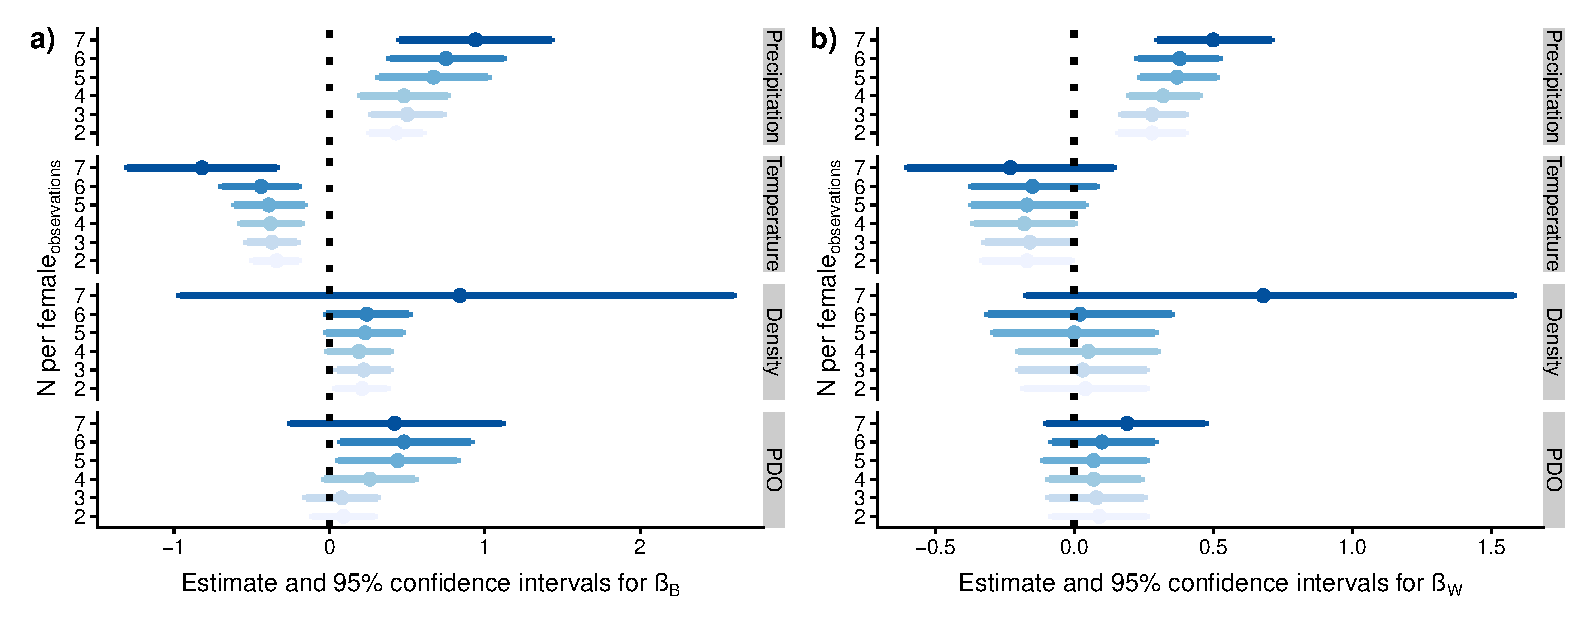
\includegraphics[width=\linewidth]{figs/annexe/ch2/ch2FigS1}
\caption[Titre de figure]{\label{ch2FigS1}Titre de figure\par{}
\smallskip		% saut de ligne entre titre et légende de figure
\normalfont{
Mean-centering was applied as suggested by \cite{Siepielski2017}}}. 
\end{figure}
\FloatBarrier
\end{landscape}

%-------------------BIBLIOGRAPHIE----------------------------
% assurez vous d’avoir un dossier avec vos listes de références par chapitre. C’est ici que chaque liste est intégrée au chapitre. 
% il faut la commande \bibliography ET \bibliographystyle pour que la liste par chapitre (avec différents styles) fonctionne. 

\singlespacing 
{\renewcommand{\bibname}{References}
\renewcommand{\bibsection}{\section{\bibname}}
\bibliography{bib/chapitre2}}
\bibliographystyle{styles/myBEAS} 
       
\setstretch{1.3}\chapter{\textbf{}} 	%titre entre {} non nécessaire car apparaît deux fois
\begin{center}
\textbf{Titre de l'article} \\
\textit{Journal} (Année), Volume (Issue): pages. \\
Auteurs 
\end{center}

\section{Titre}
\subsection{Titre}
\lipsum[2]

We followed the procedure described by \citet{Siepielski2017} as follow
\begin{align}
  \lambda_{kj} &\sim N(0,\phi^{-1}_{kj}\tau^{-1}_k)\\
  \text{where }  \phi^{-1}_{kj} &\sim \Gamma(2,1)\\
  \text{and }  \tau_k&=\prod^{k}_{l=1} \sim \Gamma(3,1)
\end{align}

In these prior definition, $\lambda$ refers to the parameters of the latent variables, where $\tau^{-1}_k$


%\FloatBarrier
\begin{figure}[htb]
\centering
%\captionsetup{format=hang,justification=raggedright,labelfont=bf, singlelinecheck = false, font=bf, labelsep=quad}
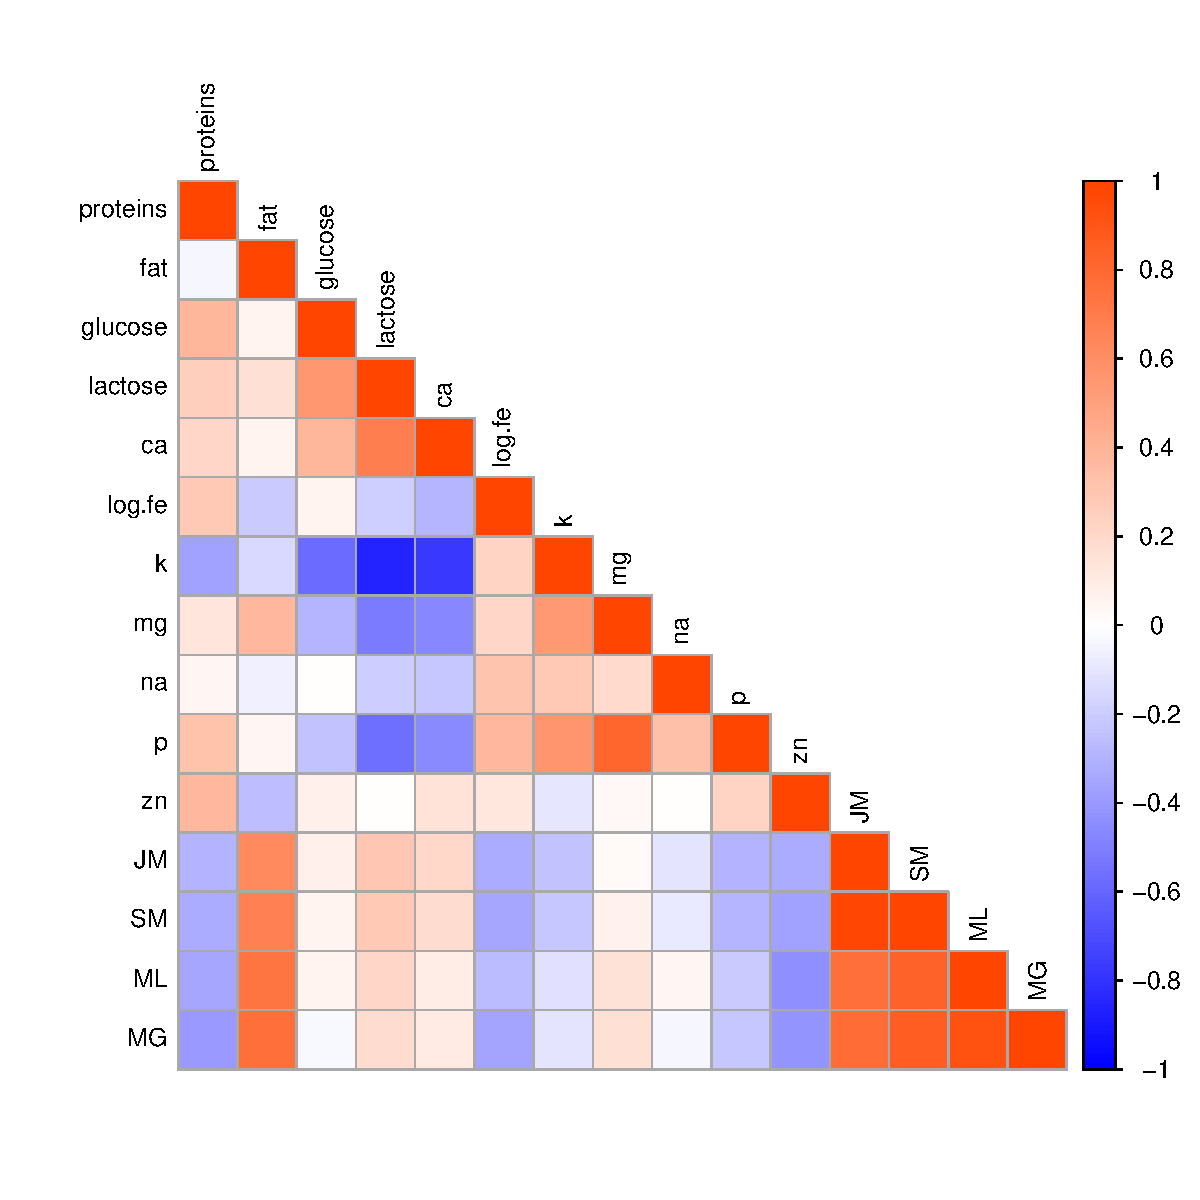
\includegraphics[width=0.85\textwidth]{figs/annexe/ch3/ch3FigS1}
\caption[Titre de figure ]{\label{ch3FigS1}Titre de figure\par{}
\smallskip		% saut de ligne entre titre et légende de figure
\normalfont{
Légende de figure}}
\end{figure}
%\FloatBarrier


% bibliographie pour l'annexe 
\singlespacing
{\renewcommand{\bibname}{References}
\renewcommand{\bibsection}{\section{\bibname}}
\bibliography{bib/chapitre2}
\bibliographystyle{styles/myBEAS} 

 


%------------------BIBLIOGRAPHIE GÉNÉRALE ----------------------------
% UTILISER LA LIGNE DE COMMANDE POUR COMPILER BIBTEX ET LATEX DANS LE BON ORDRE 

\singlespacing
\addcontentsline{toc}{chapter}{BIBLIOGRAPHIE}
{\renewcommand{\bibname}{BIBLIOGRAPHIE}
\renewcommand{\bibsection}{\chapter*{\bibname}}
\bibliography{bib/mycollection}}
\bibliographystyle{styles/myharvard} 	% modifié pour avoir les et al. en italique % attention ceci n'inclut pas tous les cas possibles (livres, chapitres de livres, etc.)



%------------------FIN DU DOCUMENT ----------------------------
% add blank page after
\nolinenumbers
\blankpage
\blankpage
\end{document}